\documentclass[10pt]{article}


\usepackage{fullpage}
\usepackage{graphicx}
\usepackage{caption}
\usepackage{subcaption}

\begin{document}

\title{MIMIC2V30 SAPS-I}
\maketitle


\begin{figure}
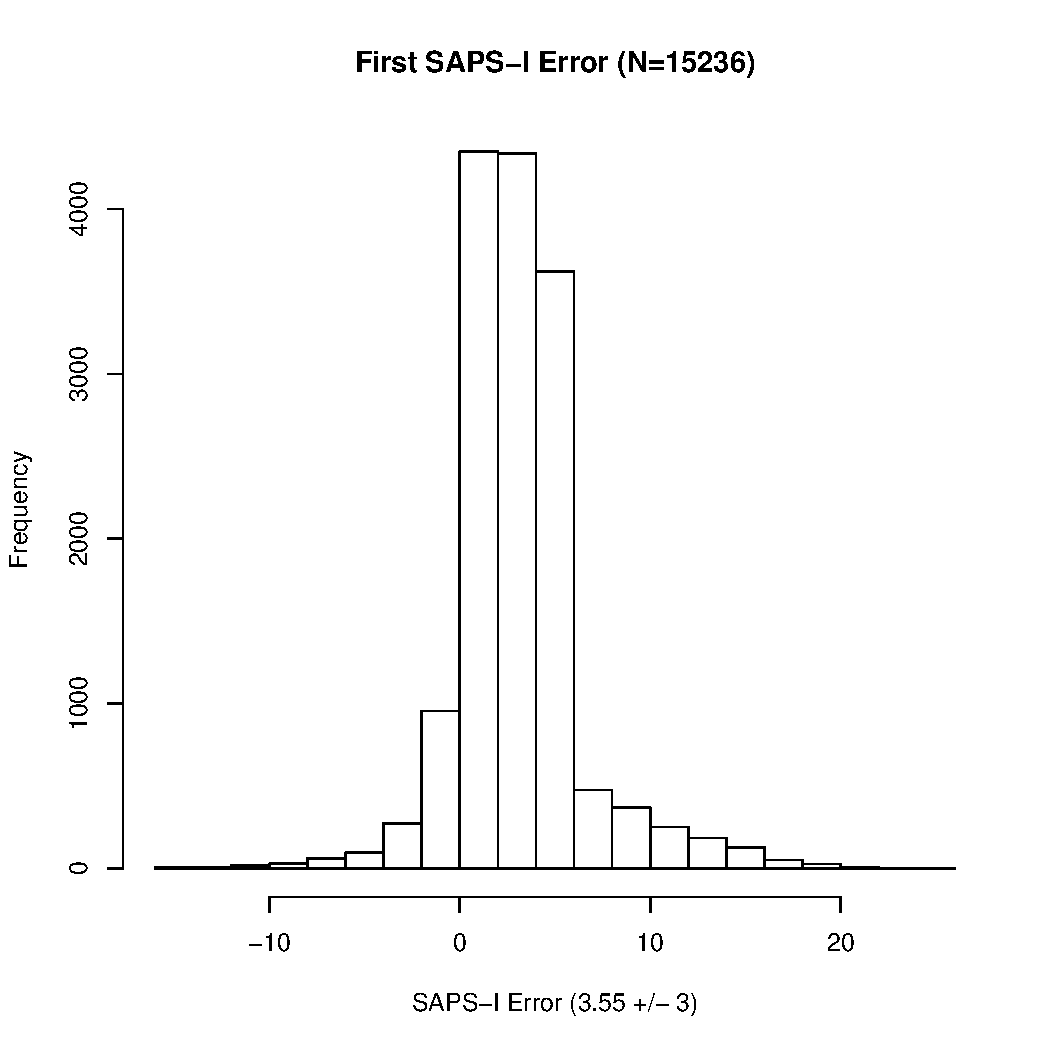
\includegraphics[width=0.45\linewidth]{../../figure/fig_hist_sapsi_first_err.pdf}
\end{figure}

\begin{figure}
\centering
        \begin{subfigure}[b]{0.5\textwidth}
                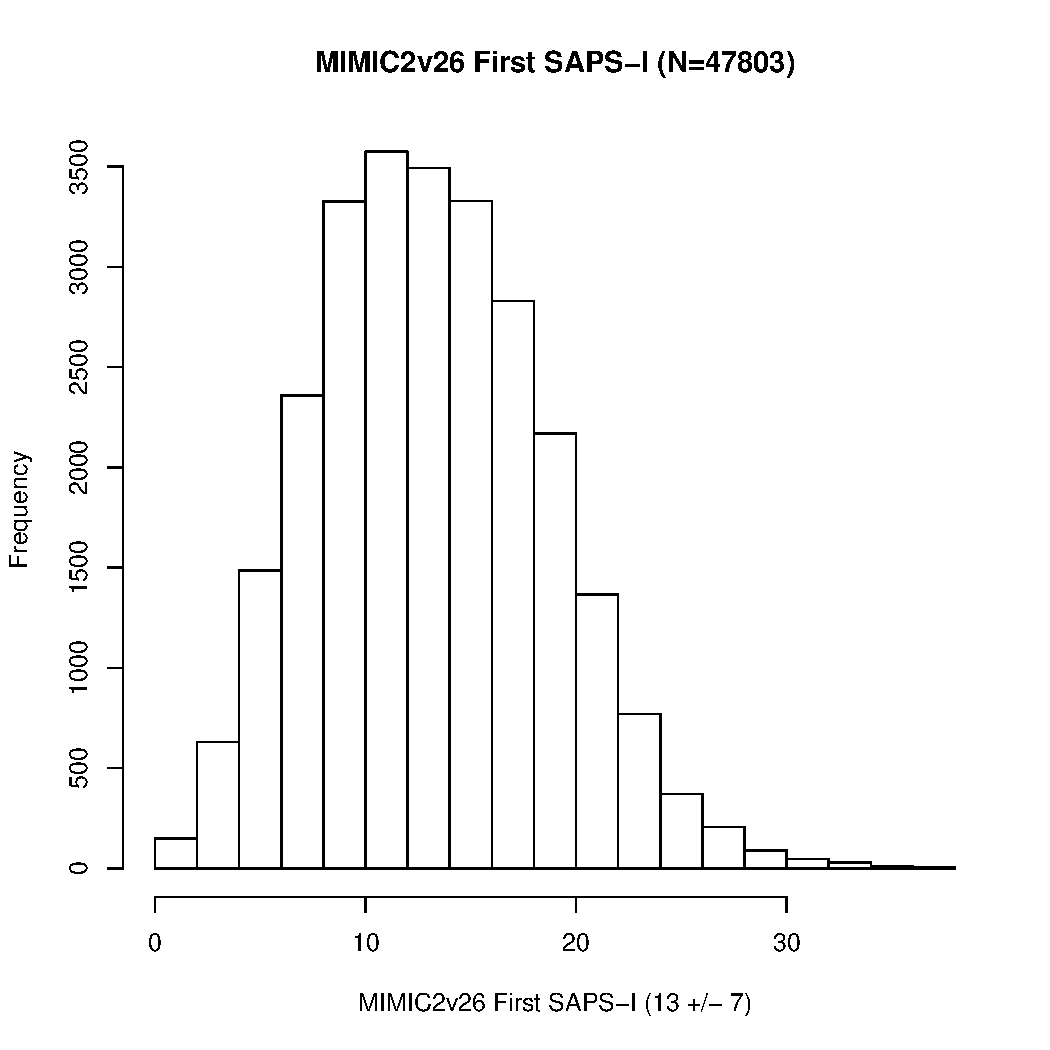
\includegraphics[width=\linewidth]{../../figure/fig_hist_sapsi_first_mimic2v26.pdf}
        \end{subfigure}%
        \begin{subfigure}[b]{0.5\textwidth}
                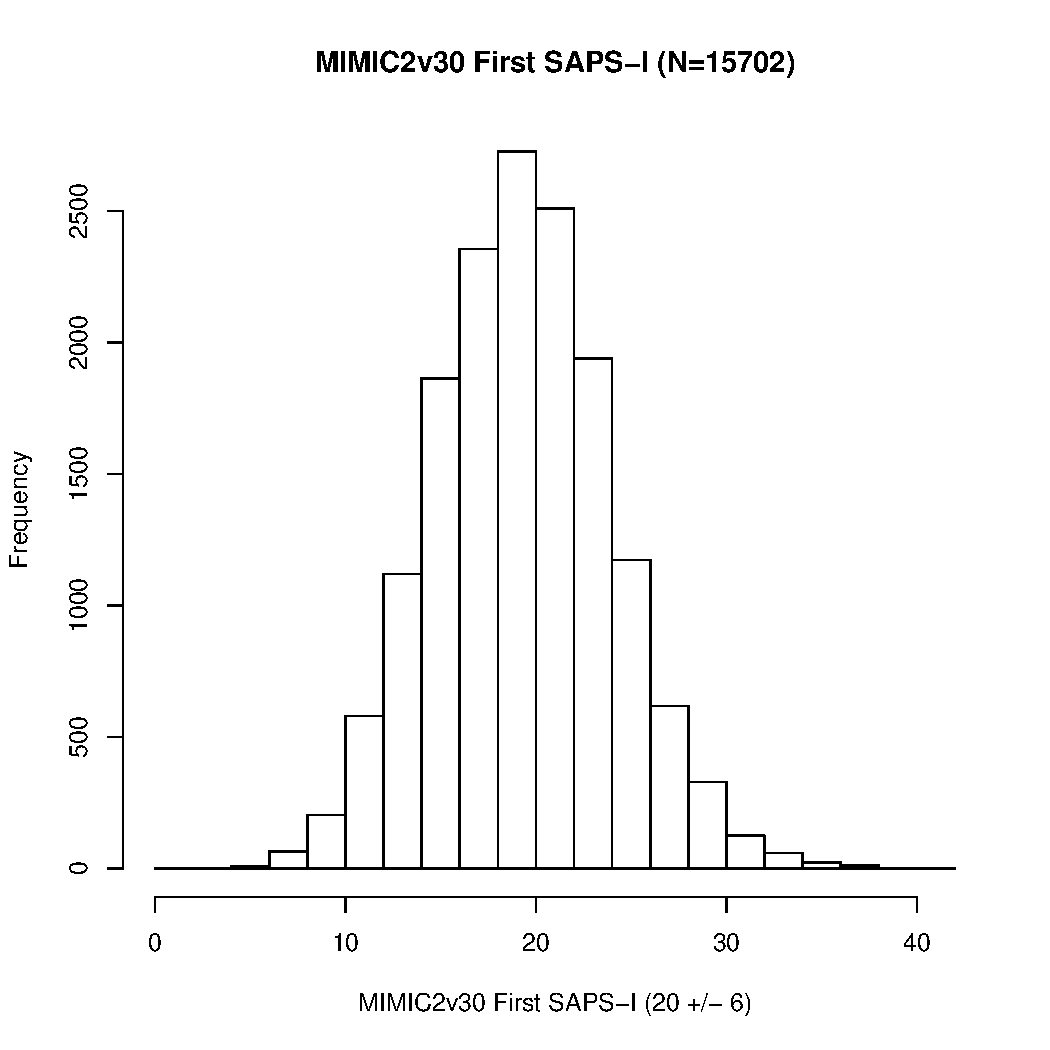
\includegraphics[width=\linewidth]{../../figure/fig_hist_sapsi_first_mimic2v30.pdf}
        \end{subfigure}
\end{figure}

\begin{figure}
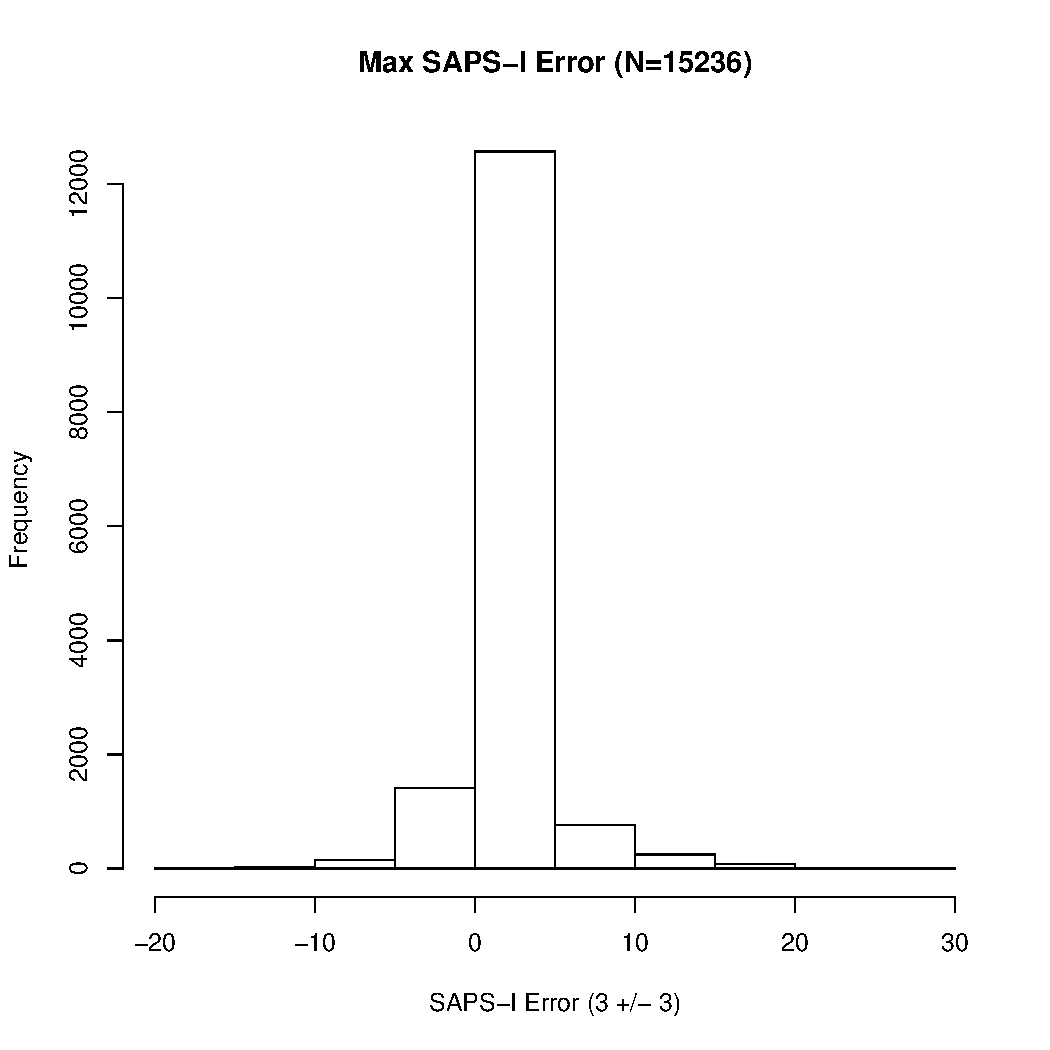
\includegraphics[width=0.45\linewidth]{../../figure/fig_hist_sapsi_max_err.pdf}
\end{figure}

\begin{figure}
        \begin{subfigure}[b]{0.5\textwidth}
                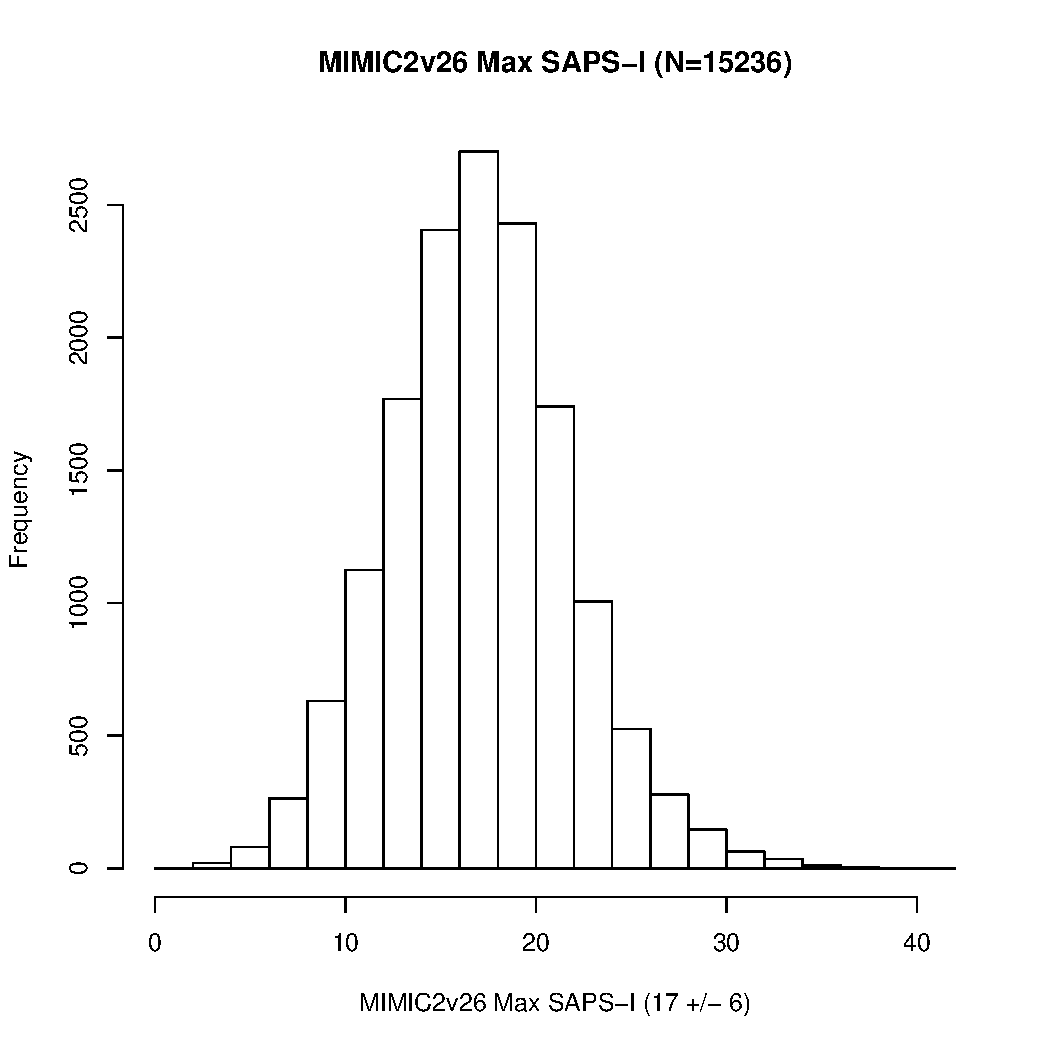
\includegraphics[width=\linewidth]{../../figure/fig_hist_sapsi_max_mimic2v26.pdf}
        \end{subfigure}%
        \begin{subfigure}[b]{0.5\textwidth}
                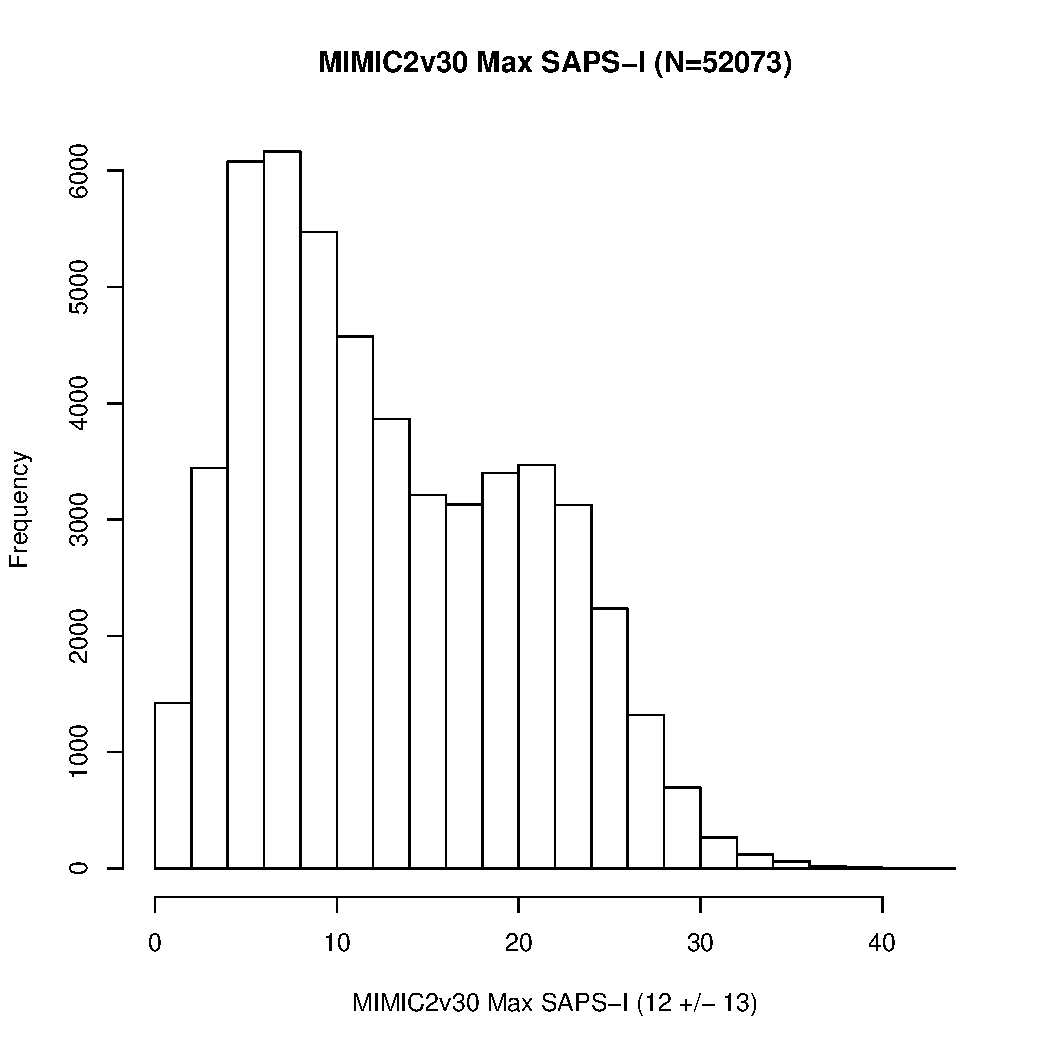
\includegraphics[width=\linewidth]{../../figure/fig_hist_sapsi_max_mimic2v30.pdf}   
        \end{subfigure}
\end{figure}


\begin{figure}
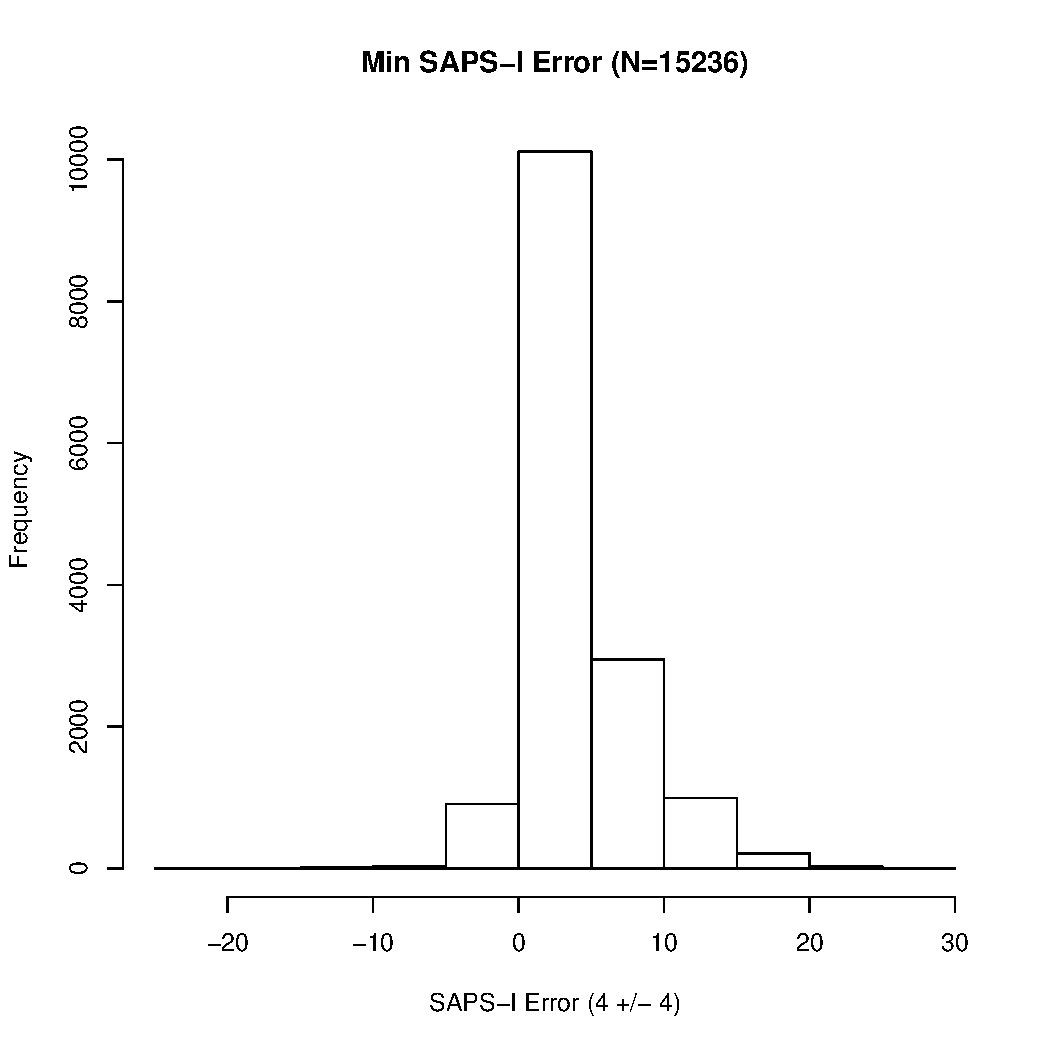
\includegraphics[width=0.45\linewidth]{../../figure/fig_hist_sapsi_min_err.pdf}
\end{figure}

\begin{figure}
        \begin{subfigure}[b]{0.5\textwidth}
                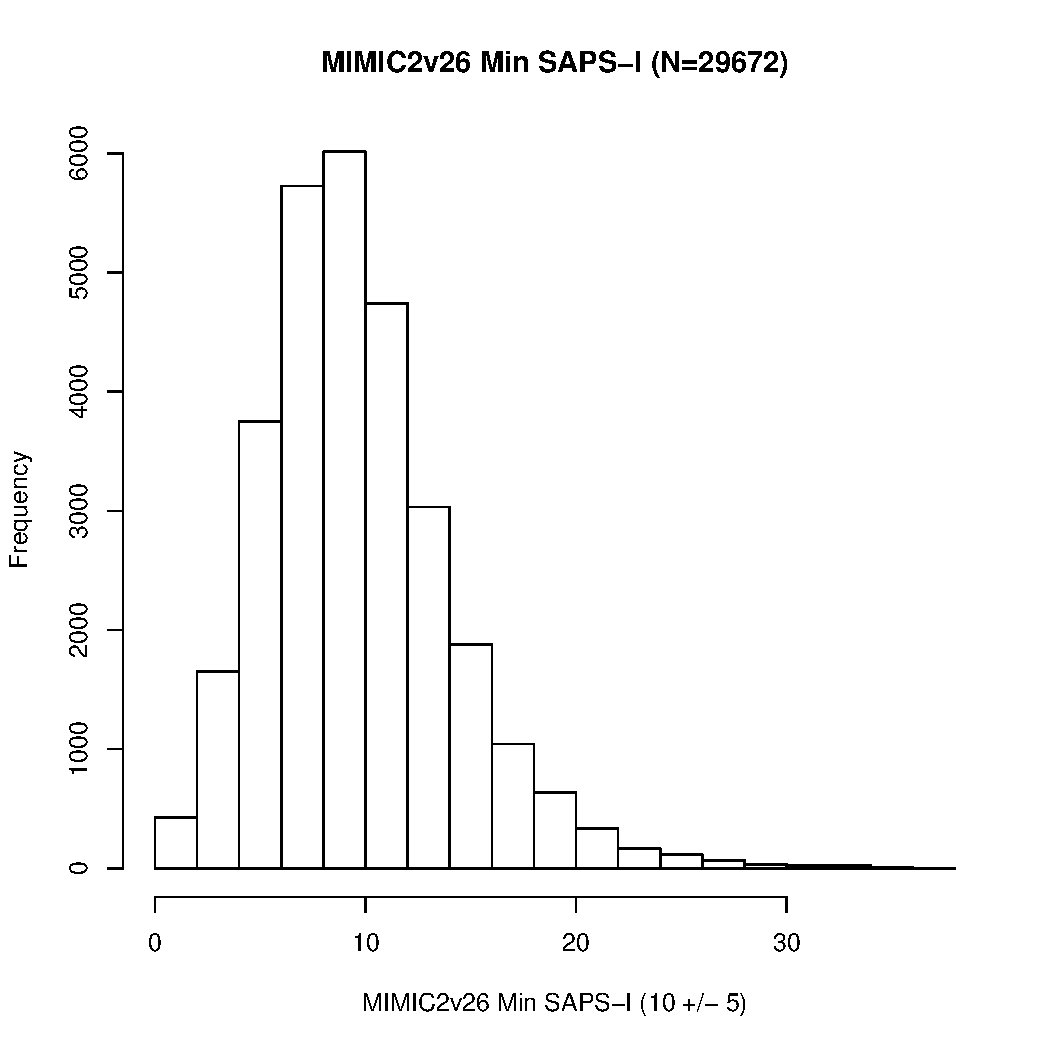
\includegraphics[width=\linewidth]{../../figure/fig_hist_sapsi_min_mimic2v26.pdf}
        \end{subfigure}%
        \begin{subfigure}[b]{0.5\textwidth}
                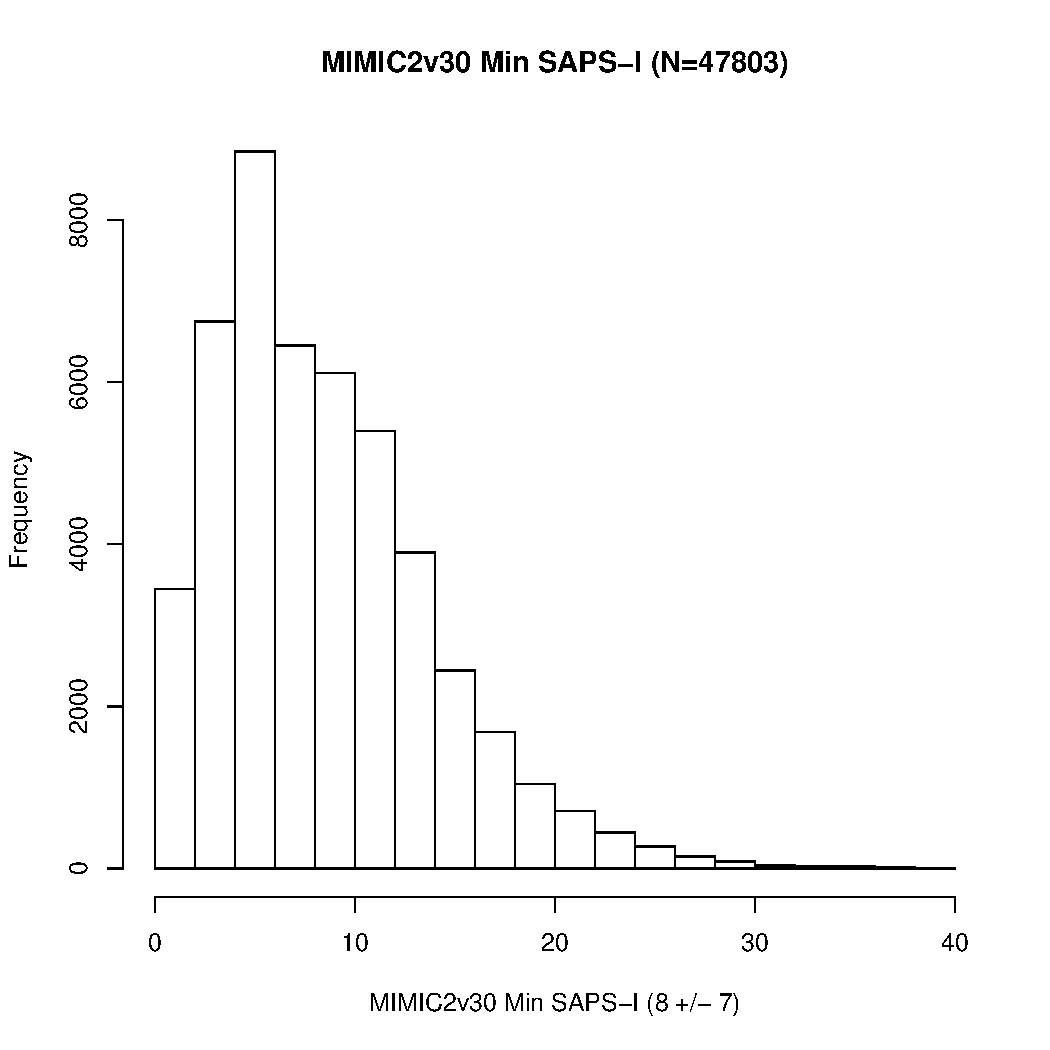
\includegraphics[width=\linewidth]{../../figure/fig_hist_sapsi_min_mimic2v30.pdf}
        \end{subfigure}
\end{figure}


\begin{figure}
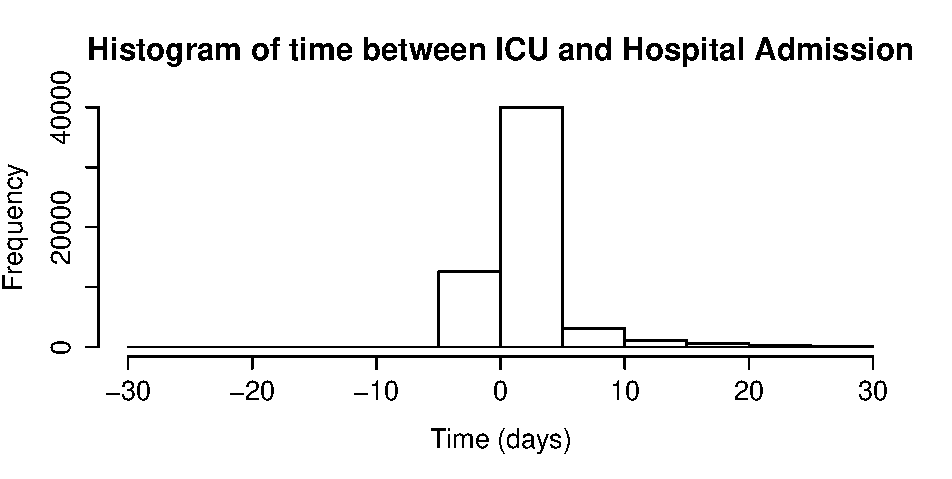
\includegraphics[width=0.45\linewidth]{../../figure/hist_hadm_dt.pdf}
\end{figure}


\end{document}
